%%%%%%%%%%%%%%%%%%%%%%%%%%%%%%%%%%%%%%%%%
% Lachaise Assignment
% LaTeX Template
% Version 1.0 (26/6/2018)
%
% This template originates from:
% http://www.LaTeXTemplates.com
%
% Authors:
% Marion Lachaise & François Févotte
% Vel (vel@LaTeXTemplates.com)
%
% License:
% CC BY-NC-SA 3.0 (http://creativecommons.org/licenses/by-nc-sa/3.0/)
% 
%%%%%%%%%%%%%%%%%%%%%%%%%%%%%%%%%%%%%%%%%

%----------------------------------------------------------------------------------------
%	PACKAGES AND OTHER DOCUMENT CONFIGURATIONS
%----------------------------------------------------------------------------------------

\documentclass{article}

%%%%%%%%%%%%%%%%%%%%%%%%%%%%%%%%%%%%%%%%%
% Lachaise Assignment
% Structure Specification File
% Version 1.0 (26/6/2018)
%
% This template originates from:
% http://www.LaTeXTemplates.com
%
% Authors:
% Marion Lachaise & François Févotte
% Vel (vel@LaTeXTemplates.com)
%
% License:
% CC BY-NC-SA 3.0 (http://creativecommons.org/licenses/by-nc-sa/3.0/)
% 
%%%%%%%%%%%%%%%%%%%%%%%%%%%%%%%%%%%%%%%%%

%----------------------------------------------------------------------------------------
%	PACKAGES AND OTHER DOCUMENT CONFIGURATIONS
%----------------------------------------------------------------------------------------

\usepackage{amsmath,amsfonts,stmaryrd,amssymb} % Math packages
\usepackage[dvipsnames]{xcolor}
\usepackage{enumerate} % Custom item numbers for enumerations
\usepackage{hyperref}
\usepackage[ruled,vlined]{algorithm2e} % Algorithms

\usepackage[framemethod=tikz]{mdframed} % Allows defining custom boxed/framed environments

\usepackage{listings} % Required for insertion of code

\newcommand{\randomcolor}{%
  \definecolor{randomcolor}{RGB}
   {
    \pdfuniformdeviate 256,
    \pdfuniformdeviate 256,
    \pdfuniformdeviate 256
   }%
  \color{randomcolor}%
}

\definecolor{codegreen}{rgb}{0,0.6,0}
\definecolor{codegray}{rgb}{0.5,0.5,0.5}
\definecolor{codepurple}{rgb}{0.58,0,0.82}
\definecolor{backcolour}{rgb}{1,1,1}
\lstdefinestyle{mystyle}{
    backgroundcolor=\color{backcolour},   
    commentstyle=\color{codegreen},
    keywordstyle=\color{magenta},
    numberstyle=\tiny\color{codegray},
    stringstyle=\color{codepurple},
    basicstyle=\ttfamily\footnotesize,
    breakatwhitespace=false,         
    breaklines=true,                 
    captionpos=b,                    
    keepspaces=true,                 
    numbers=left,                    
    numbersep=5pt,                  
    showspaces=false,                
    showstringspaces=false,
    showtabs=false,                  
    tabsize=2
}
\renewcommand{\lstlistingname}{Código}% Listing -> Algorithm
\lstset{style=mystyle}


%\usepackage{listings} % File listings, with syntax highlighting
%\lstset{
%	basicstyle=\ttfamily, % Typeset listings in monospace font
%}

%----------------------------------------------------------------------------------------
%	DOCUMENT MARGINS
%----------------------------------------------------------------------------------------

\usepackage{geometry} % Required for adjusting page dimensions and margins

\geometry{
	paper=a4paper, % Paper size, change to letterpaper for US letter size
	top=2.5cm, % Top margin
	bottom=3cm, % Bottom margin
	left=2.5cm, % Left margin
	right=2.5cm, % Right margin
	headheight=14pt, % Header height
	footskip=1.5cm, % Space from the bottom margin to the baseline of the footer
	headsep=1.2cm, % Space from the top margin to the baseline of the header
	%showframe, % Uncomment to show how the type block is set on the page
}

%----------------------------------------------------------------------------------------
%	FONTS
%----------------------------------------------------------------------------------------

\usepackage[utf8]{inputenc} % Required for inputting international characters
\usepackage[T1]{fontenc} % Output font encoding for international characters

\usepackage{XCharter} % Use the XCharter fonts
\usepackage{pgfplots}
\usepackage{multicol}
%----------------------------------------------------------------------------------------
%	COMMAND LINE ENVIRONMENT
%----------------------------------------------------------------------------------------

% Usage:
% \begin{commandline}
%	\begin{verbatim}
%		$ ls
%		
%		Applications	Desktop	...
%	\end{verbatim}
% \end{commandline}

\mdfdefinestyle{commandline}{
	leftmargin=10pt,
	rightmargin=10pt,
	innerleftmargin=15pt,
	middlelinecolor=black!50!white,
	middlelinewidth=2pt,
	frametitlerule=false,
	backgroundcolor=black!5!white,
	frametitle={Command Line},
	frametitlefont={\normalfont\sffamily\color{white}\hspace{-1em}},
	frametitlebackgroundcolor=black!50!white,
	nobreak,
}

% Define a custom environment for command-line snapshots
\newenvironment{commandline}{
	\medskip
	\begin{mdframed}[style=commandline]
}{
	\end{mdframed}
	\medskip
}

%----------------------------------------------------------------------------------------
%	FILE CONTENTS ENVIRONMENT
%----------------------------------------------------------------------------------------

% Usage:
% \begin{file}[optional filename, defaults to "File"]
%	File contents, for example, with a listings environment
% \end{file}

\mdfdefinestyle{file}{
	innertopmargin=1.6\baselineskip,
	innerbottommargin=0.8\baselineskip,
	topline=false, bottomline=false,
	leftline=false, rightline=false,
	leftmargin=2cm,
	rightmargin=2cm,
	singleextra={%
		\draw[fill=black!10!white](P)++(0,-1.2em)rectangle(P-|O);
		\node[anchor=north west]
		at(P-|O){\ttfamily\mdfilename};
		%
		\def\l{3em}
		\draw(O-|P)++(-\l,0)--++(\l,\l)--(P)--(P-|O)--(O)--cycle;
		\draw(O-|P)++(-\l,0)--++(0,\l)--++(\l,0);
	},
	nobreak,
}

% Define a custom environment for file contents
\newenvironment{file}[1][File]{ % Set the default filename to "File"
	\medskip
	\newcommand{\mdfilename}{#1}
	\begin{mdframed}[style=file]
}{
	\end{mdframed}
	\medskip
}

%----------------------------------------------------------------------------------------
%	NUMBERED QUESTIONS ENVIRONMENT
%----------------------------------------------------------------------------------------

% Usage:
% \begin{question}[optional title]
%	Question contents
% \end{question}

\mdfdefinestyle{question}{
	innertopmargin=1.2\baselineskip,
	innerbottommargin=0.8\baselineskip,
	roundcorner=5pt,
	nobreak,
	singleextra={%
		\draw(P-|O)node[xshift=1em,anchor=west,fill=white,draw,rounded corners=5pt]{%
		Pregunta \theQuestion\questionTitle};
	},
}

\newcounter{Question} % Stores the current question number that gets iterated with each new question

% Define a custom environment for numbered questions
\newenvironment{question}[1][\unskip]{
	\bigskip
	\stepcounter{Question}
	\newcommand{\questionTitle}{~#1}
	\begin{mdframed}[style=question]
}{
	\end{mdframed}
	\medskip
}

%----------------------------------------------------------------------------------------
%	WARNING TEXT ENVIRONMENT
%----------------------------------------------------------------------------------------

% Usage:
% \begin{warn}[optional title, defaults to "Warning:"]
%	Contents
% \end{warn}

\mdfdefinestyle{warning}{
	topline=false, bottomline=false,
	leftline=false, rightline=false,
	nobreak,
	singleextra={%
		\draw(P-|O)++(-0.5em,0)node(tmp1){};
		\draw(P-|O)++(0.5em,0)node(tmp2){};
		\fill[black,rotate around={45:(P-|O)}](tmp1)rectangle(tmp2);
		\node at(P-|O){\color{white}\scriptsize\bf !};
		\draw[very thick](P-|O)++(0,-1em)--(O);%--(O-|P);
	}
}

% Define a custom environment for warning text
\newenvironment{warn}[1][Warning:]{ % Set the default warning to "Warning:"
	\medskip
	\begin{mdframed}[style=warning]
		\noindent{\textbf{#1}}
}{
	\end{mdframed}
}

%----------------------------------------------------------------------------------------
%	INFORMATION ENVIRONMENT
%----------------------------------------------------------------------------------------

% Usage:
% \begin{info}[optional title, defaults to "Info:"]
% 	contents
% 	\end{info}

\mdfdefinestyle{info}{%
	topline=false, bottomline=false,
	leftline=false, rightline=false,
	nobreak,
	singleextra={%
		\fill[black](P-|O)circle[radius=0.4em];
		\node at(P-|O){\color{white}\scriptsize\bf i};
		\draw[very thick](P-|O)++(0,-0.8em)--(O);%--(O-|P);
	}
}

% Define a custom environment for information
\newenvironment{info}[1][Info:]{ % Set the default title to "Info:"
	\medskip
	\begin{mdframed}[style=info]
		\noindent{\textbf{#1}}
}{
	\end{mdframed}
}
 % Include the file specifying the document structure and custom commands

%----------------------------------------------------------------------------------------
%	ASSIGNMENT INFORMATION
%----------------------------------------------------------------------------------------

\title{ITC-ADA-C1-2023: Assignment \#5} % Title of the assignment

\author{Luis Ballado\\ \texttt{luis.ballado@cinvestav.mx}} % Author name and email address

\date{CINVESTAV UNIDAD TAMAULIPAS --- \today} % University, school and/or department name(s) and a date

%----------------------------------------------------------------------------------------

\begin{document}

\maketitle % Print the title

%----------------------------------------------------------------------------------------
%	INTRODUCTION
%----------------------------------------------------------------------------------------

%--- cambiar estilo de secciones
\titleformat{\section}  % which section command to format
  {\fontsize{12}{12}\bfseries} % format for whole line
  {\thesection} % how to show number
  {1em} % space between number and text
  {} % formatting for just the text
  [] % formatting for after the text

\section{Diseñe e implemente los algoritmos necesarios para resolver eficientemente los dos incisos del problema 4.13 de la página 127 del libro de Dasgupta, Papadimitriou y Vazirani. Analice matemáticamente la complejidad temporal de sus algoritmos.}

\begin{question}
  \textbf{Dado un conjunto de ciudades, junto con el patrón de carreteras entre ellas, en forma de un gráfico no dirigido G=(V,E). Cada tramo de la carretera $e \in E$ conecta dos de las ciudades, y usted conoce su longitud en millas. Suponga que quiere ir de la ciudad $s$ a la ciudad $t$ . Pero hay un problema, su coche solo puede contener suficiente gasolina para cubrir L millas. Hay gasolineras en cada ciudad, pero no entre ciudades. Por lo tanto, solo se puede tomar una ruta si cada una de sus aristas tiene una longitud de $l_{e} \neq L$}

  a) Dada la limitación en la capacidad del tanque de combustible de su coche, muestre cómo determinar en tiempo lineal si existe una ruta factible de $s$ a $t$\\
  b) Ahora planea comprar un coche nuevo y desea saber cuál es el tanque mínimo de combustible que se necesita para viajar de $s$ a $t$. Proponga un algoritmo O(($|$V$|$ + $|$E$|$) log$|$V$|$) para determinar esto.
\end{question}
  
%se responde aquí
\textit{a) Para determinar si existe un camino de s $\implies$ t con las limitantes del tanque de gasolina del carro, podemos hacer uso del algoritmo de BFS; manteniendo un rastro de las ciudades visitadas y revisando cuando el costo de cada arista es menor o igual que la capacidad del tanque.\\\\ Si la corrida del algoritmo BFS logra alcanzar la ciudad destino, podemos decir que existe una ruta con la capacidad del tanque.\\\\ Comenzamos en la ciudad s y visitamos todas las ciudades adjacentes a ella que se puedan llegar con L millas, marcamos la ciudad como visitada y la agregamos a la cola, continuaremos este proceso hasta llegar a la ciudad destino.\\\\ La complejidad del algoritmo es \textbf{O($|$V$|$+$|$E$|$)} ya que visitamos todos los vertices y aristas una vez}\\\\

\textit{b) Para determinar la capacidad mínima, que necesitamos para viajar entre las ciudades de interés, podemos hacer uso de una búsqueda binaria comenzando con un mínimo de cero y una máxima distancia entre las dos ciudades en el grafo. Para así, haciendo uso de la búsqueda con las capacidades del tanque, se busca una ruta entre ciudades.\\\\ Para conocer si existe una ruta dada la capacidad del tanque, se hace uso nuevamente del algoritmo BFS. \\Si existe, repetiremos la búsqueda binaria hasta encontrar la capacidad mínima que nos permita llegar de la ciudad s $implies$ t. \\\\ Dado que la búsqueda binaria corre en \textbf{O(log(v))} para cada iteración y cada iteración necesita correr el algoritmo BFS en el grafo cuyo costo es \textbf{O($|$V$|$+$|$E$|$)}, teniendo una complejidad total de \textbf{O($|$V$|$+$|$E$|$)log$|$V$|$)} }

\subsection{Análisis Matemático}

Análisis de entrada para cada iteración de la búsqueda binaria:\\
Primera iteración : $n$\\
Segunda iteración : $\frac{n}{2}$\\
Tercera iteración : $\frac{\frac{n}{2}}{2} = \frac{n}{2^{2}}$
Iteración n : $\frac{n}{2^{k}}$, \\
sabemos que después de n iteraciones no se necesita hacer alguna comparación $\frac{n}{2^{k}} = 1 \implies n = 2^{k}$ Aplicando log en ambos lados: \\
$log_{2}(n) = log_{2}(2^{k})$\\
$log_{2}(n) = k*log_{2}(2) \implies k = log_{2}(n)$ \\\\

Análisis de BFS:\\

Cada vértice vecino se inserta a la cola si no ha sido visitado. Esto se hace con las aristas adjacentes al vértice. Cada vértice visitado se marca como visitado, por lo tanto, cada vértice se visita una sola vez y se verifican todas las aristas adjacentes al vértice. Haciendo que su complejidad sea: $O(|V|+|E|)$

\subsection{Implementación y corridas}

\href{https://github.com/luisballado/ADA/tree/main/practice_code/tarea5/car_highways}{ver código en github}\\

\begin{figure}[h]
  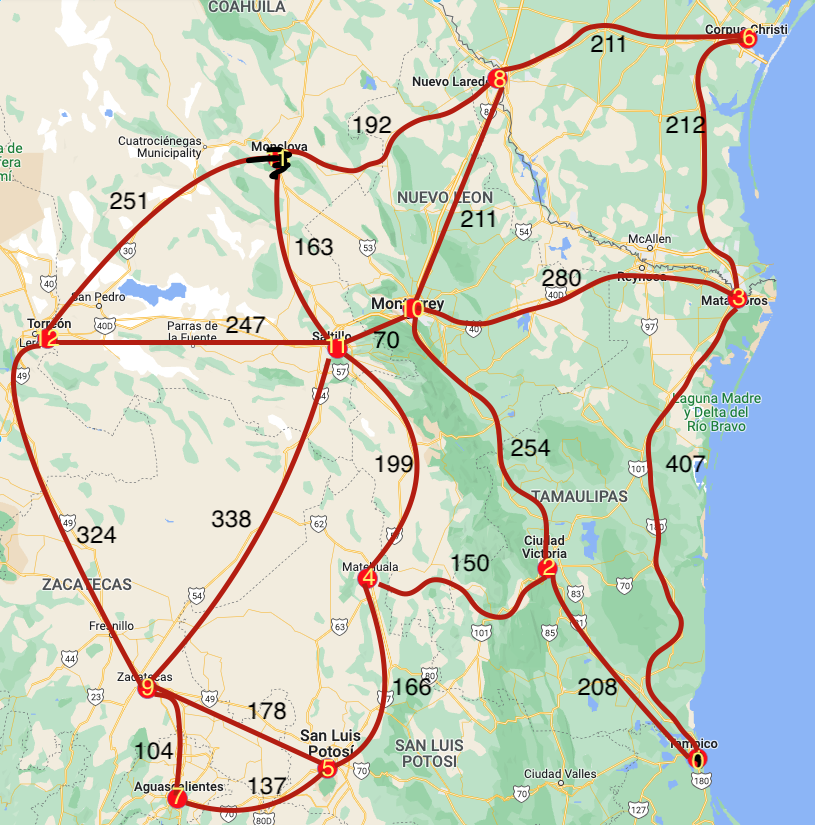
\includegraphics[scale=0.5]{grafo.png}
  \centering
\end{figure}

Partiendo del siguiente grafo propuesto, dónde nuestra ciudad de origen es Tampico (soy de Tampico) y nuestra ciudad destino es Monclova. Cada arista representa aproximadamente la distancia en kilometros de ciudad a ciudad.\\
Nuestro grafo cuenta con 13 vértices, y 20 aristas y queremos saber si existe una ruta de Tampico (Vértice 0) a Monclova (Vértice 1).\\\\
La representación del grafo se presenta en el archivo \href{https://github.com/luisballado/ADA/blob/main/practice_code/tarea5/car_highways/data.txt}{data.txt}\\

Ejecutar desde una terminal\\\\

El archivo data.txt contiene los datos de
\begin{itemize}
\item \textbf{número de ciudades, número de caminos}
\item \textbf{Seguido de las aristas (ciudad origen-ciudad destino) y sus respectivos pesos}
\item \textbf{ciudad origen, ciudad destino}
\end{itemize}

% Command-line "screenshot"
\begin{commandline}
\begin{verbatim}
  $ g++ -std=c++11 cars_highways.cpp -o cars_highways
  $ ./cars_highways < data.txt
  Existe una ruta de la ciudad 0 a la ciudad 1
  Considerar un tanque que cubra 208 km para viajar de la ciudad 0 a la ciudad 1
\end{verbatim}
\end{commandline}

Si forzamos los datos desconectando a Cd. Victoria del grafo en la arista Tampico-Cd.Victoria, forzaremos que la ruta sea vía Matamoros convirtiendose ese tramo en el mas costoso que debe ser considerado para la adquisición del nuevo auto. \href{https://github.com/luisballado/ADA/blob/main/practice_code/tarea5/car_highways/data2.txt}{data2.txt}\\

\begin{commandline}
\begin{verbatim}
  $ g++ -std=c++11 cars_highways.cpp -o cars_highways
  $ ./cars_highways < data2.txt
  Existe una ruta de la ciudad 0 a la ciudad 1
  Considerar un tanque que cubra 407 km para viajar de la ciudad 0 a la ciudad 1
\end{verbatim}
\end{commandline}


\newpage
\section{Diseñe e implemente un algoritmo que permita resolver eficientemente el inciso (a) del problema 4.21 de la página 130 del libro de Dasgupta, Papadimitriou y Vazirani. Analice matemáticamente la complejidad temporal de su algoritmo.}

\begin{question}
  \textbf{Los algoritmos de ruta más corta se pueden aplicar en el comercio de divisas. Sea $c_{1}$ , $c_{2}$ , ... , $c_{n}$ ser varias monedas; por ejemplo, $c_{1}$ podría ser dólares, $c_{2}$ libras y $c_{3}$ liras. Para dos monedas cualesquiera $c_{i}$ y $c_{j}$ , hay un tipo de cambio $r_{i,j}$ ; esto significa que puede comprar $r_{i,j}$ unidades de moneda $c_{j}$ en cambiar por una unidad de $c_{i}$. Estos tipos de cambio satisfacen la condición de que $r_{i,j} * r_{j,i} < 1$, de modo que si comienza con una unidad de moneda $c_{i}$ , la cambia a moneda $c_{j}$ y luego vuelve a convertirla a moneda $c_{i}$ , terminas con menos de una unidad de moneda $c_{i}$ (la diferencia es el costo de la transacción).}

  a) Realice un algoritmo eficiente: dado un conjunto de tipos de cambio $r_{i,j}$, y dos monedas s y t, encuentre la secuencia más ventajosa de cambios de moneda para convertir la moneda s en la moneda t. Represente las monedas y tasas en un grafo cuyas longitudes son números reales.
  
\end{question}

\textit{Podemos resolver el problema haciendo uso del algoritmo de Dijkstra, encontrando el camino más corto en un grafo con pesos. Representando las divisas como los nodos del grafo y las tasas de cambio como aristas con pesos. Especificamente para cada par de divisas $c_{i}$ y $c_{j}$, podemos crear una arista de $c_{i}$ a $c_{j}$ con un peso de $-log(r_{i},j)$, se hace uso del algoritmo negativo ya que la tasa de intercambio satisface la condición de $r_{i,j}*r_{j,i} < 1$\\\\ La idea es transformar las tasas de intercambio en retornos logarítmicos. Esta propiedad es de ayuda, ya que nos permite hacer uso de algoritmos para encontrar el camino más corto (Dijkstra) y así encontrar el camino con mejores ganancias. \\ Con los pesos de las aristas representados como logaritmos negativos convirtiendo el problema con pesos no negativos, de esta forma es posible hacer uso del algoritmo de Dijkstra, de otra forma se usaria el algoritmo de Bellman Ford para aristas negativas.\\\\ La complejidad es \textbf{O($|$E$|$+$|$V$|$log$|$V$|$)}, hay que señalar que a raíz de que hacemos uso de logaritmos, necesitamos tener cuidado con aristas que sean cercanas a cero.}

\subsection{Análisis matemático}

Dado el grafo representado como una lista de adjacencia y una cola de prioridad, se calcula su complejidad:

\begin{enumerate}
\item Tomará $O(|V|)$ inicializar la cola de prioridad dados $|V|$ vértices.
\item Con la representación del grafo como lista de adjacencia, todos los vértices del grafo se pueden recorrer usando BFS. Ya que se itera sobre todos los vértices vecinos, actualizando su distancia. Esto toma $O(|E|)$
\item El tiempo para cada iteración es $O(|V|)$, ya que los vértices son removidos de la cola en cada ciclo.
\item La cola de prioridad nos permite extraer el nodo con minima distancia. Esto toma $O(log(|V|))$
\item Su complejidad está dada por $O(|V|)+O(|E|*log|V|)+O(|V|*log|V|) \implies O((|E|+|V|)*log|V|) = O(|E|*log|V|)$, dado que $|E|>= |V| - 1$.
\end{enumerate}
\newpage
\subsection{Implementación}
\href{https://github.com/luisballado/ADA/tree/main/practice_code/tarea5/currency_trading}{ver código en github}\\

Ejecutar desde una terminal\\\\

El archivo data.txt contiene los datos de
\begin{itemize}
\item \textbf{monedas, tasas de cambio}
\item \textbf{moneda origen, moneda destino, tasa de cambio}
\item \textbf{moneda origen, moneda destino}
\end{itemize}

% Command-line "screenshot"
\begin{commandline}
\begin{verbatim}
  $ g++ -std=c++11 currency_trading.cpp -o currency_trading
  $ ./currency_trading < data.txt
  El intercambio de 0 a 3 es 0.4
\end{verbatim}
\end{commandline}

\newpage
\section{Referencias}
Dijkstra Complexity - \url{https://www.baeldung.com/cs/dijkstra-time-complexity}\\\\
Bellman-Ford to Find Arbitrage Condition in Forex Trading - \url{https://informatika.stei.itb.ac.id/~rinaldi.munir/Matdis/2019-2020/Makalah2019/13518058.pdf}\\\\
C++ Currency Arbitrage Bellman-Ford- \url{https://cppsecrets.com/users/166319711511599105105995564103109971051084699111109/C00-Currency-Arbitrage.php}\\\\
Búsqueda Binaria - \url{https://www.tutorialspoint.com/data_structures_algorithms/binary_search_algorithm.htm}\\\\
Búsqueda Binaria - \url{https://medium.com/@Emmitta/b%C3%BAsqueda-binaria-c6187323cd72}\\\\
Rate of return - \url{https://en.wikipedia.org/wiki/Rate_of_return}\\\\
Returns and Log Returns - \url{https://gregorygundersen.com/blog/2022/02/06/log-returns}\\\\
Analysis of breadth-first search algorithm - \url{https://www.khanacademy.org/computing/computer-science/algorithms/breadth-first-search/a/analysis-of-breadth-first-search}\\\\
COMPSCI 311: Introduction to Algorithms - \\\url{https://people.cs.umass.edu/~marius/class/cs311-fa18/lec15-nup.pdf}\\\\
Arbitrage as a Shortest-Path Problem - \\\url{https://hackernoon.com/arbitrage-as-a-shortest-path-problem-u2l34ow}\\\\
Currency Arbitrage using Bellman Ford Algorithm - \\\url{https://anilpai.medium.com/currency-arbitrage-using-bellman-ford-algorithm-8938dcea56ea}\\\\
Temas de C++ - \\\url{https://www.fing.edu.uy/tecnoinf/mvd/cursos/eda/material/teo/EDA-teorico14.pdf}\\\\
Array de vectores en C++ - \url{https://www.geeksforgeeks.org/array-of-vectors-in-c-stl/}\\\\
Vectores C++ - \url{https://www.programiz.com/cpp-programming/vectors}\\\\
Implementacion de un grafo para programacion competitiva \\ \url{https://www.geeksforgeeks.org/graph-implementation-using-stl-for-competitive-programming-set-1-dfs-of-unweighted-and-undirected/}

\end{document}

